\documentclass[11pt,letterpaper]{article}
\usepackage[margin=.65in,top=.78in,bottom=.65in]{geometry}
\usepackage[T1]{fontenc}
\usepackage{lmodern,tikz,fancyhdr}
\renewcommand{\familydefault}{\sfdefault}
\pagestyle{fancy}\fancyhf{}
\fancyhead[L]{\small Week 74 / Doubling elevators / Stride strips}
\fancyfoot[L]{\small Bellingham Math Circle / Week 74 / GGT74-M-v1}
\fancyfoot[R]{\small\thepage}
\renewcommand{\headrulewidth}{0pt}\renewcommand{\footrulewidth}{0pt}
\setlength{\parindent}{0pt}\setlength{\parskip}{6pt}
% One stride strip. The ticks are 1, 2, 4, 8 and 16 board dot spaces (0.23 in each)
% from the 0 tick: 0.23, 0.46, 0.92, 1.84 and 3.68 in.
\newcommand{\stridestrip}[1]{%
 \begin{scope}[yshift=#1]
  \draw[line width=.5pt] (-.25,0) rectangle (4.0,-.62);
  \draw[line width=1.2pt] (0,0)--(0,-.34);
  \foreach \s in {1,2,4,8,16} {\draw[line width=.6pt] ({.23*\s},0)--({.23*\s},-.34);}
  \foreach \s in {0,1,2,4,8,16} {\node[below,font=\footnotesize,inner sep=1.5pt] at ({.23*\s},-.34) {\s};}
 \end{scope}}
\begin{document}
Adults: print at 100\% (Actual size), on card stock if you have it, and cut out one strip for each pair. Check one strip on a board: with its 0 on a dot, the 16 tick should sit on the dot 16 spaces to the right. For R, put the 0 on the marker and move to the tick for the level's step. For L, put that tick on the marker and move to the 0. The strips have not yet been tried with children.

\vspace{.15in}
\begin{center}
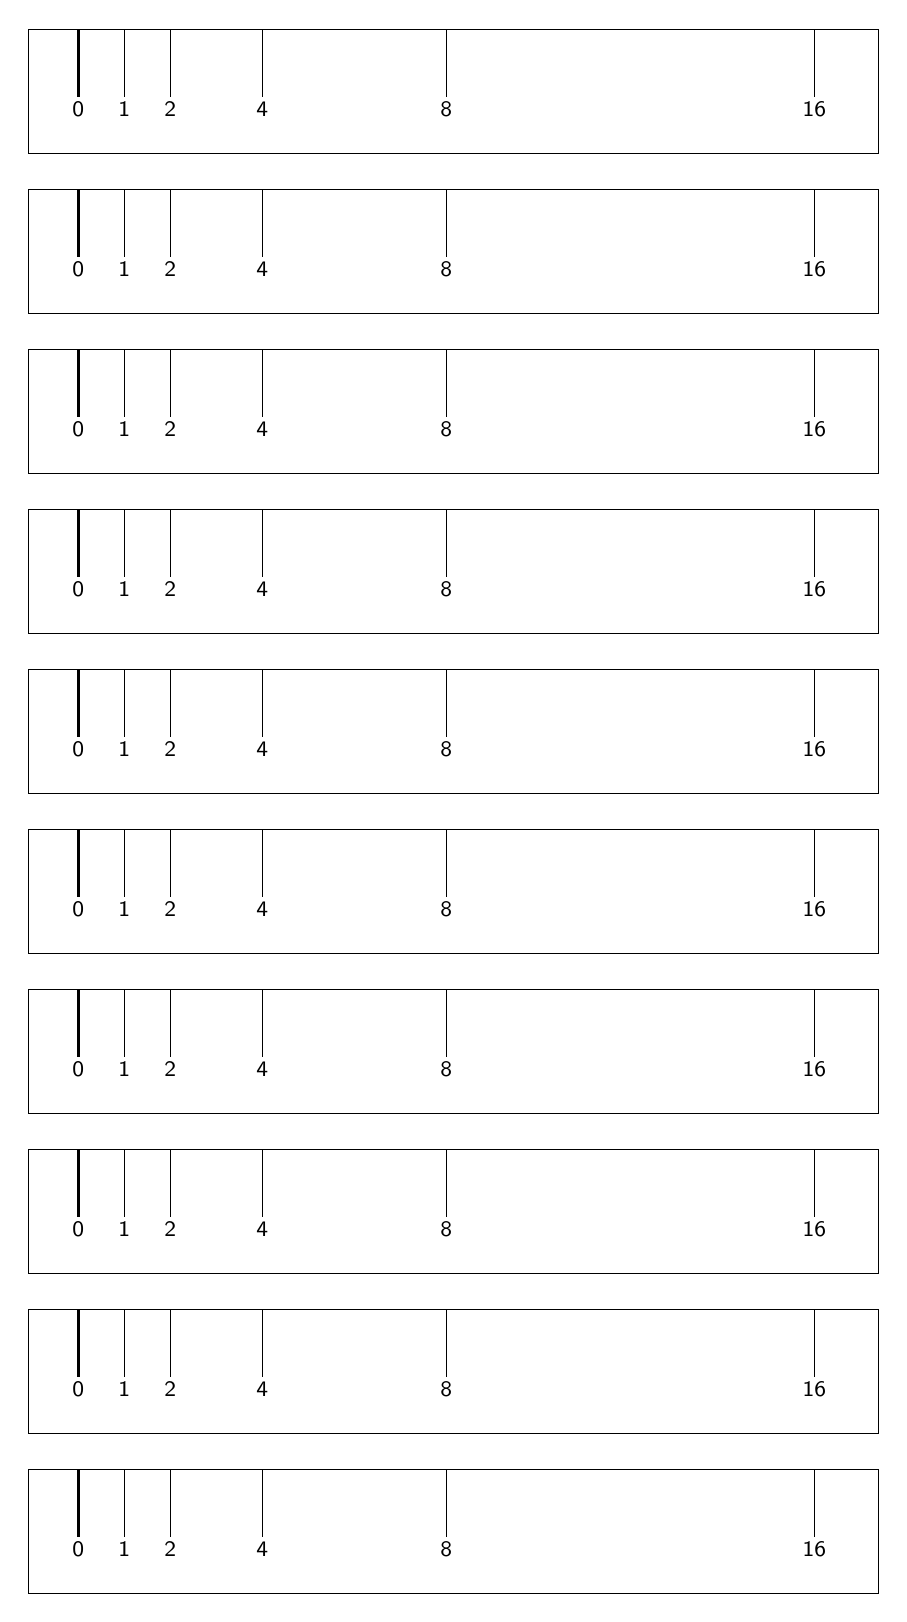
\begin{tikzpicture}[x=1in,y=1in]
\foreach \i in {0,...,9} {\stridestrip{-\i*.8in}}
\end{tikzpicture}
\end{center}
\end{document}
